% due July 8
\DocumentMetadata{
  lang=en,
  tagging=on,
  pdfstandard=ua-2,
%  check-tagging-status,
  tagging-setup={
%    math/alt/use,
    math/setup=mathml-SE
  }
}
\documentclass{ltx-talk}

% see https://github.com/josephwright/ltx-talk/issues/233
\ExplSyntaxOn
\keys_define:nn { talk / metadata } { unknown .code:n = {} }
\ExplSyntaxOff

\date{TUG 2026}
\title[pdftitle={Accessible PDFs}]{Accessible PDFs}
% without pdftitle,
% the PDF's title ends up being what was last used by \maketitle
\author[pdfauthor={Timothy Prescott},short-author={Tim Prescott}]
 {Timothy Prescott (\TeX.SE: \texttt{teepeemm})}
\institute{University of North Dakota}

% abstract for textbook:
%A guideline in the United States requires that
%\acro{PDF}s created after April 2026 must be accessible to visually
%impaired users. We discuss how we updated a custom three semester
%calculus book to be accessible, including what we did, the challenges we
%faced, how we verified accessibility, and what remains to be done. We
%also discuss necessary adaptations to satisfy a common accessibility
%checker available in several \acro{LMS}s.

% 30 minutes including questions

\usepackage{booktabs}
\usepackage{siunitx}
\usepackage{emoji}
\usepackage{tikz-cd}
\usepackage{pgfplots}
\usepackage{listings}
\usepackage[normalem]{ulem}
\usepackage{multicol}

\DeclareMathOperator{\coker}{coker}
\pgfplotsset{compat=1.18}

\newcommand{\apex}{\texorpdfstring{A\kern -.1em \lower -.5ex\hbox{P}\kern -.25em\lower .5ex\hbox{E}\kern -.1em X}{APEX}}

\ProvideDocumentEnvironment{tcb@manual@entry}{}{}{} % needed for the next line
\usepackage{tagpdfdocu-patches}% needed to make listings work properly

\makeatletter
\lstset{
  columns=fullflexible,
  keepspaces=true,
  commentstyle=\slshape,
  basicstyle=\ttfamily
  \lst@ifdisplaystyle\small\fi,
  language={[LaTeX]TeX}
}
\makeatother

\newcommand{\cs}[1]{\texttt{\textbackslash #1}}
\newcommand{\tubbraced}[1]{\texttt{\{#1\}}}
\newcommand{\meta}[1]{\ensuremath{\langle}%
 \ifmmode\expandafter\mbox\fi{\itshape #1\/}%
 \ensuremath{\rangle}%
}

%\providecolor{maybeUNDgreen}{Hsb}{146,1,0.62}
\providecolor{maybeUNDgreen}{Hsb}{146,1,0.53}

\EditInstance{header}{std}{
    background-color = maybeUNDgreen,
    color            = white,
}

\DeclareInstance{footer-element}{frameoftotal}{talk}{}
\ExpandArgs{c}\newcommand{@frameoftotal}{%
  \arabic{frame}/\RefProperty{lastpage}{totalframes}
}
\EditInstance{footer}{std}{
  separator     = \hfill,
  element-order = {date, author, title, frameoftotal},
}

\DeclareInstance{titlepage-element}{titlegraphic}{talk}{}
% department logo obtained locally
% other graphics from https://campus.und.edu/brand/downloads.html
% primary logotype, full color, svg converted to pdf
\ExpandArgs{c}\newcommand{@titlegraphic}{%
  \addvspace{\medskipamount}
  
\includegraphics[
    actualtext={University of North Dakota, Mathematics \& Statistics},
    width=5cm
  ]{MathStats-CMYK_primary.jpg}% logotype-full
  \addvspace{\smallskipamount}
}
% flame logo, white, digital png
\newsavebox\logobox
%\savebox\logobox{\includegraphics[artifact, height=2ex]{example-image}}
\savebox\logobox{%
  
\includegraphics[artifact, height=\baselineskip]{flame-w-rgb}}
\AddToHook{shipout/foreground}{%
  \put(\paperwidth - \wd\logobox - 10mm,
       -8.5mm){\usebox\logobox}} % -\ht\logobox
%\NewCommandCopy\oldframetitle\frametitle
%\RenewDocumentCommand{\frametitle}{m}{%
%  \oldframetitle{#1\hfill
%    
\includegraphics[height=2ex,artifact]{flame-w-rgb}%
%  }%
%}

\begin{document}

\title[short-title={Accessible PDF Textbook}]
 {Converting a PDF Textbook to be Accessible}

\begin{frame}[name=titleslide]
\renewcommand{\ULthickness}{2pt}
\maketitle[
  element-order = {title, author, titlegraphic, date},
  framestyle = plain
]
\end{frame}

\begin{frame}
\frametitle{A strangely sporadic timeline}
\newlength{\maxwidth}
\setlength{\maxwidth}{\widthof{2024-04-26}}
\begin{description}[
  label-width=\maxwidth+1em,
  label-align=left,
%  left-margin=10em,
  left-margin=\maxwidth+1em,
]
\item[1978] \TeX
\item[1990] Americans with Disabilities Act (ADA). \\
Title II: Government entities may not discriminate\\
against those with disabilities.
\item[1993] PDF
\item[2016] University of North Dakota adopts \apex\ Calculus\\
3 semesters, 1100 pages, \texttt{CC-BY-NC 4.0}.
\item[2017--2020] PDF 2.0 (better math support).
\item[2019] \LaTeX\ team begins improving accessibility in earnest
\item[2024-04-26] US Dept of Justice: ADA Title II means that\\
public entities must make PDFs accessible.\\
Most entities get two years.  We (DoJ) get three years.
\item[2026-04-20] Everyone gets an extra year.
\end{description}
\end{frame}

\begin{frame}
\frametitle{Basic outline of accessibilizing}
\begin{itemize}[item-vspace=\bigskipamount]
\item Preamble
\item Images
\item Tables
\item All else
\end{itemize}
\end{frame}

\begin{frame}
\frametitle{Basic table of accessibilizing}
\sisetup{table-format=3}
\tagpdfsetup{table/header-rows={1,2}}
\begin{tabular}{ l SSS S @{}}\toprule
Topic & \multicolumn{3}{c}{Time spent (\%)} & {How accessible} \\
& {on the textbook} & {today} & {on your own} & {(\%)} \\
%\midrule
\cmidrule(r){1-1}\cmidrule(lr){2-4}\cmidrule(l){5-5}
\textcolor{structure}{\labelitemi}~ Preamble & 3 & 10 & {<1} & 85 \\\addlinespace
\textcolor{structure}{\labelitemi}~ Images & 20 & 40 & 25 & 5 \\\addlinespace
\textcolor{structure}{\labelitemi}~ Tables & 17 & 10 & 25 & 5 \\\addlinespace
\textcolor{structure}{\labelitemi}~ All else & 60 & 40 & 50 & 5 \\
%\midrule
\cmidrule(r){1-1}\cmidrule(lr){2-4}\cmidrule(l){5-5}
 & 100 & 100 & 100 & 100\\\bottomrule
\end{tabular}
\end{frame}

\begin{frame*}
\frametitle{TL;DR}
Update \LaTeX
\begin{lstlisting}
\DocumentMetadata{
  lang=en,
  tagging=on,
  pdfstandard=ua-2,
% check-tagging-status,
  tagging-setup={
%    math/alt/use,        % <=> Formulas must have description/alt text
    math/setup=mathml-SE
  }
}
\documentclass{...}
\usepackage{unicode-math}
\end{lstlisting}
compile with Lua\LaTeX, and most of the work is done\\
\texttt{texdoc documentmetadata-support-code}
\end{frame*}

%\section{How to \TeX\ an accessible PDF}

\begin{frame*}
\frametitle{Basic idea}
Use good \LaTeX\ so that the output looks how you want it\\
\emph{and the input reflects the meaning.}
\begin{itemize}
\item Aim for a clean log
\item Don't use tabular to position boxes.
\item Make use of \emph{semantic} macros and environments:\\
Bad: \verb|\textbf{Example 3.1.4 Finding Extreme Values}|\\
Good: \verb|\begin{example}[Finding Extreme Values]|
% \end{example}
\item Prefer custom environments over macros:\\
Bad: \verb|\begin{enumerate}\renewcommand\theenumi\roman{enumi}|\\
Good: \verb|\begin{romanlist}|\\
Better: \verb|\begin{exerciselist}|
%\end{exerciselist}\end{romanlist}\end{enumerate}
\end{itemize}
\end{frame*}

\begin{frame}
\frametitle{What else to do --- images}
\begin{itemize}
\ttfamily
\item\cs{includegraphics}[\textbf{alt=\tubbraced{...}}]
\item\cs{tikz}[\textbf{alt=\tubbraced{...}}]
\item\cs{begin}\tubbraced{tikzpicture}[\textbf{alt=\tubbraced{...}}]
\item\cs{begin}\tubbraced{picture}[\textbf{alt=\tubbraced{...}}]
\end{itemize}
%Keep it brief and objective; exposition won't be seen by most readers\\
Alternatives to {\bfseries\ttfamily alt=\tubbraced{...}} are
\begin{itemize}
\item {\bfseries\ttfamily artifact} (image is decorative only)\quad
\colorbox{maybeUNDgreen}{
\includegraphics[height=\baselineskip,artifact]{flame-w-rgb}}
\item {\bfseries\ttfamily actualtext=\tubbraced{...}}
(image is text in disguise)
\quad
\raisebox{-.8\height}{%
  
\includegraphics[
    actualtext={University of North Dakota, Mathematics \& Statistics},
    width=5cm
  ]{MathStats-CMYK_primary.jpg}% logotype-full
}
\end{itemize}
%\\
%PAC objects to a bug in pgfplots.
\end{frame}

\begin{frame*}
\frametitle{Alt text}
\begin{itemize}
\item Usually not seen
\item Brief, specific, accurate, objective, neutral
\item What does my audience need from this picture?
\item How would I tell someone to draw this picture?
\item Do not begin with ``image''
\item Do not repeat the caption
\item At most 120 characters or 1--2 sentences.\\
If not possible, have the alt text point to a separately written description
\smallskip
%\item Backup method: \verb|\setkeys{Gin}{alt={...}}|
\item \!\!``Formulas need alt text'' $\leftrightarrow$ option
\texttt{math/alt/use} \emoji{thumbsdown}
\item Have someone else write the alt text?
\end{itemize}
\end{frame*}

\begin{frame}
\frametitle{Alt text problem 1}
``What alt text would you give for the snake lemma?''\bigskip
\AddToHookNext{env/tikzcd/begin}{\MathCollectFalse}
\begin{tikzcd}[
    ampersand replacement = \&,
    alt={A complicated commutative diagram.},
    every label/.append style = {font = \small}
%    font=\footnotesize,
%    row sep=small,
%    column sep=tiny,
%    cramped,
  ]
  \& \& \ker(a) \ar{r} \ar{d}
  \& \ker(b)\ar{r} \ar{d}
  \& \ker(c) \ar{d}   %\arrow[ddll,"\delta",rounded corners
  \& \&\\
  \& \& A \ar{r}{f} \ar{dd}[near end]{a}
  \& B \ar{r}{g} \ar{dd}[near end]{b}
  \& C \ar{r}\ar{dd}[near end]{c} \& 0 \& ~\\
  \& \& \& ~ \& \& \ar[r, phantom, ""{coordinate, name=Y}] \&~\\
  ~\& \ar[l, phantom, ""{coordinate, name=Z}] 0 \ar{r}
  \& A' \ar{r}{f'} \ar{d}
  \& B' \ar{r}{g'} \ar{d}
  \& C' \ar{d} \& \& \\
  \& \&
  \ar[from=uuuurr, "d", crossing over, rounded corners,
      to path={ -- ([xshift=2ex]\tikztostart.east)
                -| (Y) [near end]\tikztonodes
                -| (Z) [near end]\tikztonodes
                |- ([xshift=-2ex]\tikztotarget.west)
                -- (\tikztotarget)}
     ]\coker(a)\ar{r}
  \& \coker(b) \ar{r}
  \& \coker(c) \& \&
\end{tikzcd}
\end{frame}

\begin{frame}
\frametitle{Alt text problem 1b}
\begin{minipage}{\textheight}
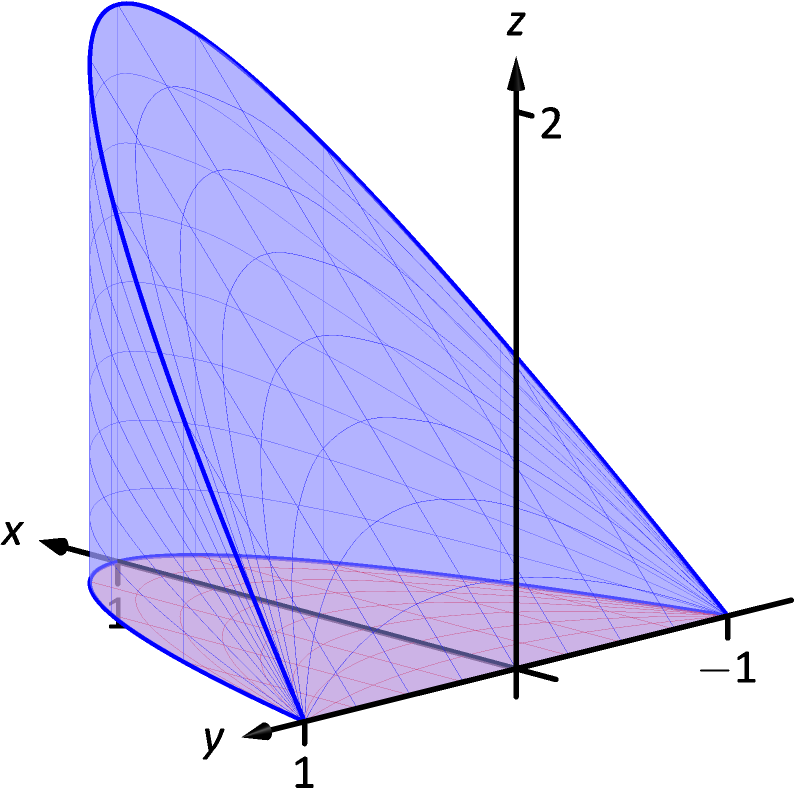
\includegraphics[width=\textheight,alt={An interactive 3d shape from the textbook.}]{figdivthm_space2_3D}
\end{minipage}\quad
\begin{minipage}{.4\textwidth}
Textbook feature:\smallskip\\
Asymptote + media9 \\
\null\quad\textrightarrow\ interactive 3d graphics
\end{minipage}
\end{frame}

\begin{frame}
\frametitle{Alt text problem 2}
  Exercise: Describe this function, identifying limiting values, intercepts
  and their degree, critical and inflection points,
  and regions where the function is increasing, decreasing, and
  concave up or down.\\
  \begin{tikzpicture}
  \begin{axis}[xmin=-2,xmax=2,ymin=-.1,ymax=1.6,width=\linewidth,
  axis x line=center,axis y line=center,axis equal image]
    \draw(-2,0.5)--(-1,1)circle(.04);
    \draw[fill=black](-1,0)circle(.04);
    \addplot[domain=-1:2,smooth]{.5*(x+1)*(x-1)^2};
  \end{axis}
  \end{tikzpicture}
\end{frame}

\begin{frame}
\frametitle{What else to do --- tables}
\begin{itemize}
\item\texttt{\cs{tagpdfsetup}\tubbraced{table/header-rows=\tubbraced{...},\\
\hphantom{XtagpdfsetupX}table/header-columns=\tubbraced{...}}\\
\qquad\qquad \textrm{outside of the} tabular\\
\qquad\qquad \textrm{(lasts until the group} \cs{ends})}
\item\texttt{\cs{tagpdfsetup}\tubbraced{table/multirow=\tubbraced{\meta{number of rows}}}} 
\item Interface will probably change
\item \texttt{texdoc latex-lab-table}
%\item Need to work around a PAC bug
%\item And PAC still doesn't like multi(row/column) in the data
\end{itemize}
\end{frame}

\begin{frame}<1>[name=stycls,tag-slides=1-2]
\frametitle{Replacements \& adjustments}
\begin{itemize}
\item Some packages need some (or a lot of) help (tcolorbox, qrcode, media9, \ldots)\\
use option \texttt{check-tagging-status} or\\
\url{https://latex3.github.io/tagging-project/tagging-status/}
\item enumitem \& enumerate \textrightarrow\ enumext or templates (\texttt{texdoc blocks-doc})
\item \sout{margin[fit|fix|note] \textrightarrow\ margin[alia|par]}
\item titlesec \textrightarrow
\begin{itemize}
\item \cs{@startsection} (\texttt{texdoc latex2e}, \S6.8)
\item templates (\texttt{texdoc latex-lab-sec-template})
\end{itemize}
\renewcommand{\ULthickness}{1pt}
\item<1-|alert@2> Beamer \textrightarrow\ ltx-talk \alt<2>{\sout{(later)}}{(later)}
\end{itemize}
\end{frame}

%\section{Testing}

\begin{frame}
\frametitle{Tools}
To verify that a PDF is accessible:
\begin{description}
%\item[Ally, Siteimprove:] (Commercial addons)
%\begin{itemize}
%\item[\emoji{thumbsup}] easy to pass, checks color contrast
%\item[\emoji{thumbsdown}] too easy, false negatives
%\end{itemize}
\item[Screen reader:] (NVDA or JAWS) and (Adobe, FoxIt, or Firefox)
\item[veraPDF:] \url{https://verapdf.org/software}
\begin{itemize}
\item[\emoji{thumbsup}] has command line version; \LaTeX\ team
\item[\emoji{thumbsdown}] no GUI for PDF errors
\end{itemize}
\item[PDFix:] \url{https://pdfix.net}
\begin{itemize}
\item[\emoji{thumbsup}] GUI
\item[\emoji{thumbsdown}] no command line
\end{itemize}
%\item[PAC:] \url{https://pac.pdf-accessibility.org/en}
%\begin{itemize}
%\item[\emoji{thumbsdown}] Windows only; maxes out at UA-1/1.7; bug with tabular headers
%\item[\emoji{thumbsup}\emoji{thumbsdown}] more thorough (pgfplots, multi[row|column])
%\end{itemize}
\end{description}
\end{frame}

% cut for MAA
%\section{Tools}

\begin{frame}
\frametitle{veraPDF --- \url{https://verapdf.org/software}}
%\centering
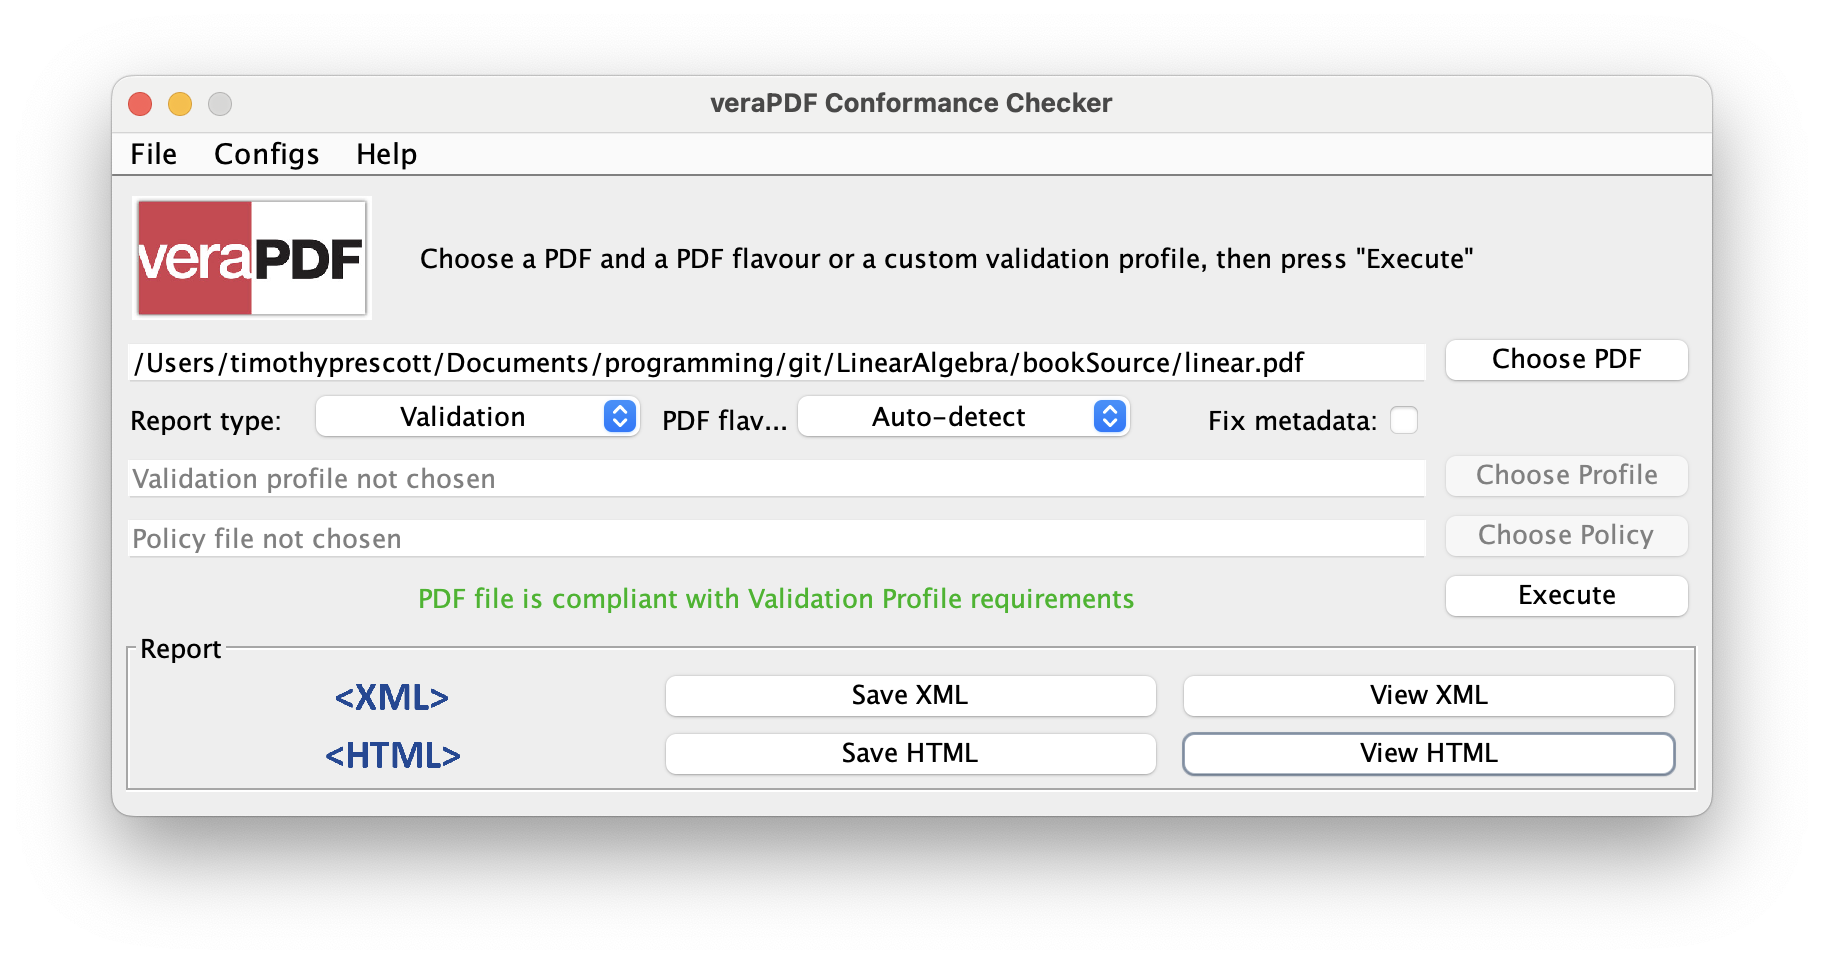
\includegraphics[alt={Screenshot of veraPDF},height=\textheight]{veraPdfScreenshot}
\end{frame}

\begin{frame*}
\frametitle{veraPDF --- example error}
\begin{verbatim}
root/
  document[0]/
  StructTreeRoot[0](5 0 obj PDStructTreeRoot)/
  K[0](22 0 obj SEDocument Document)/
  K[2130](24072 0 obj SESect figures)/
  K[71](102535 0 obj SEAside float)
\end{verbatim}
\end{frame*}

\begin{frame}
\frametitle{PDFix --- \url{https://pdfix.net}}
%\centering
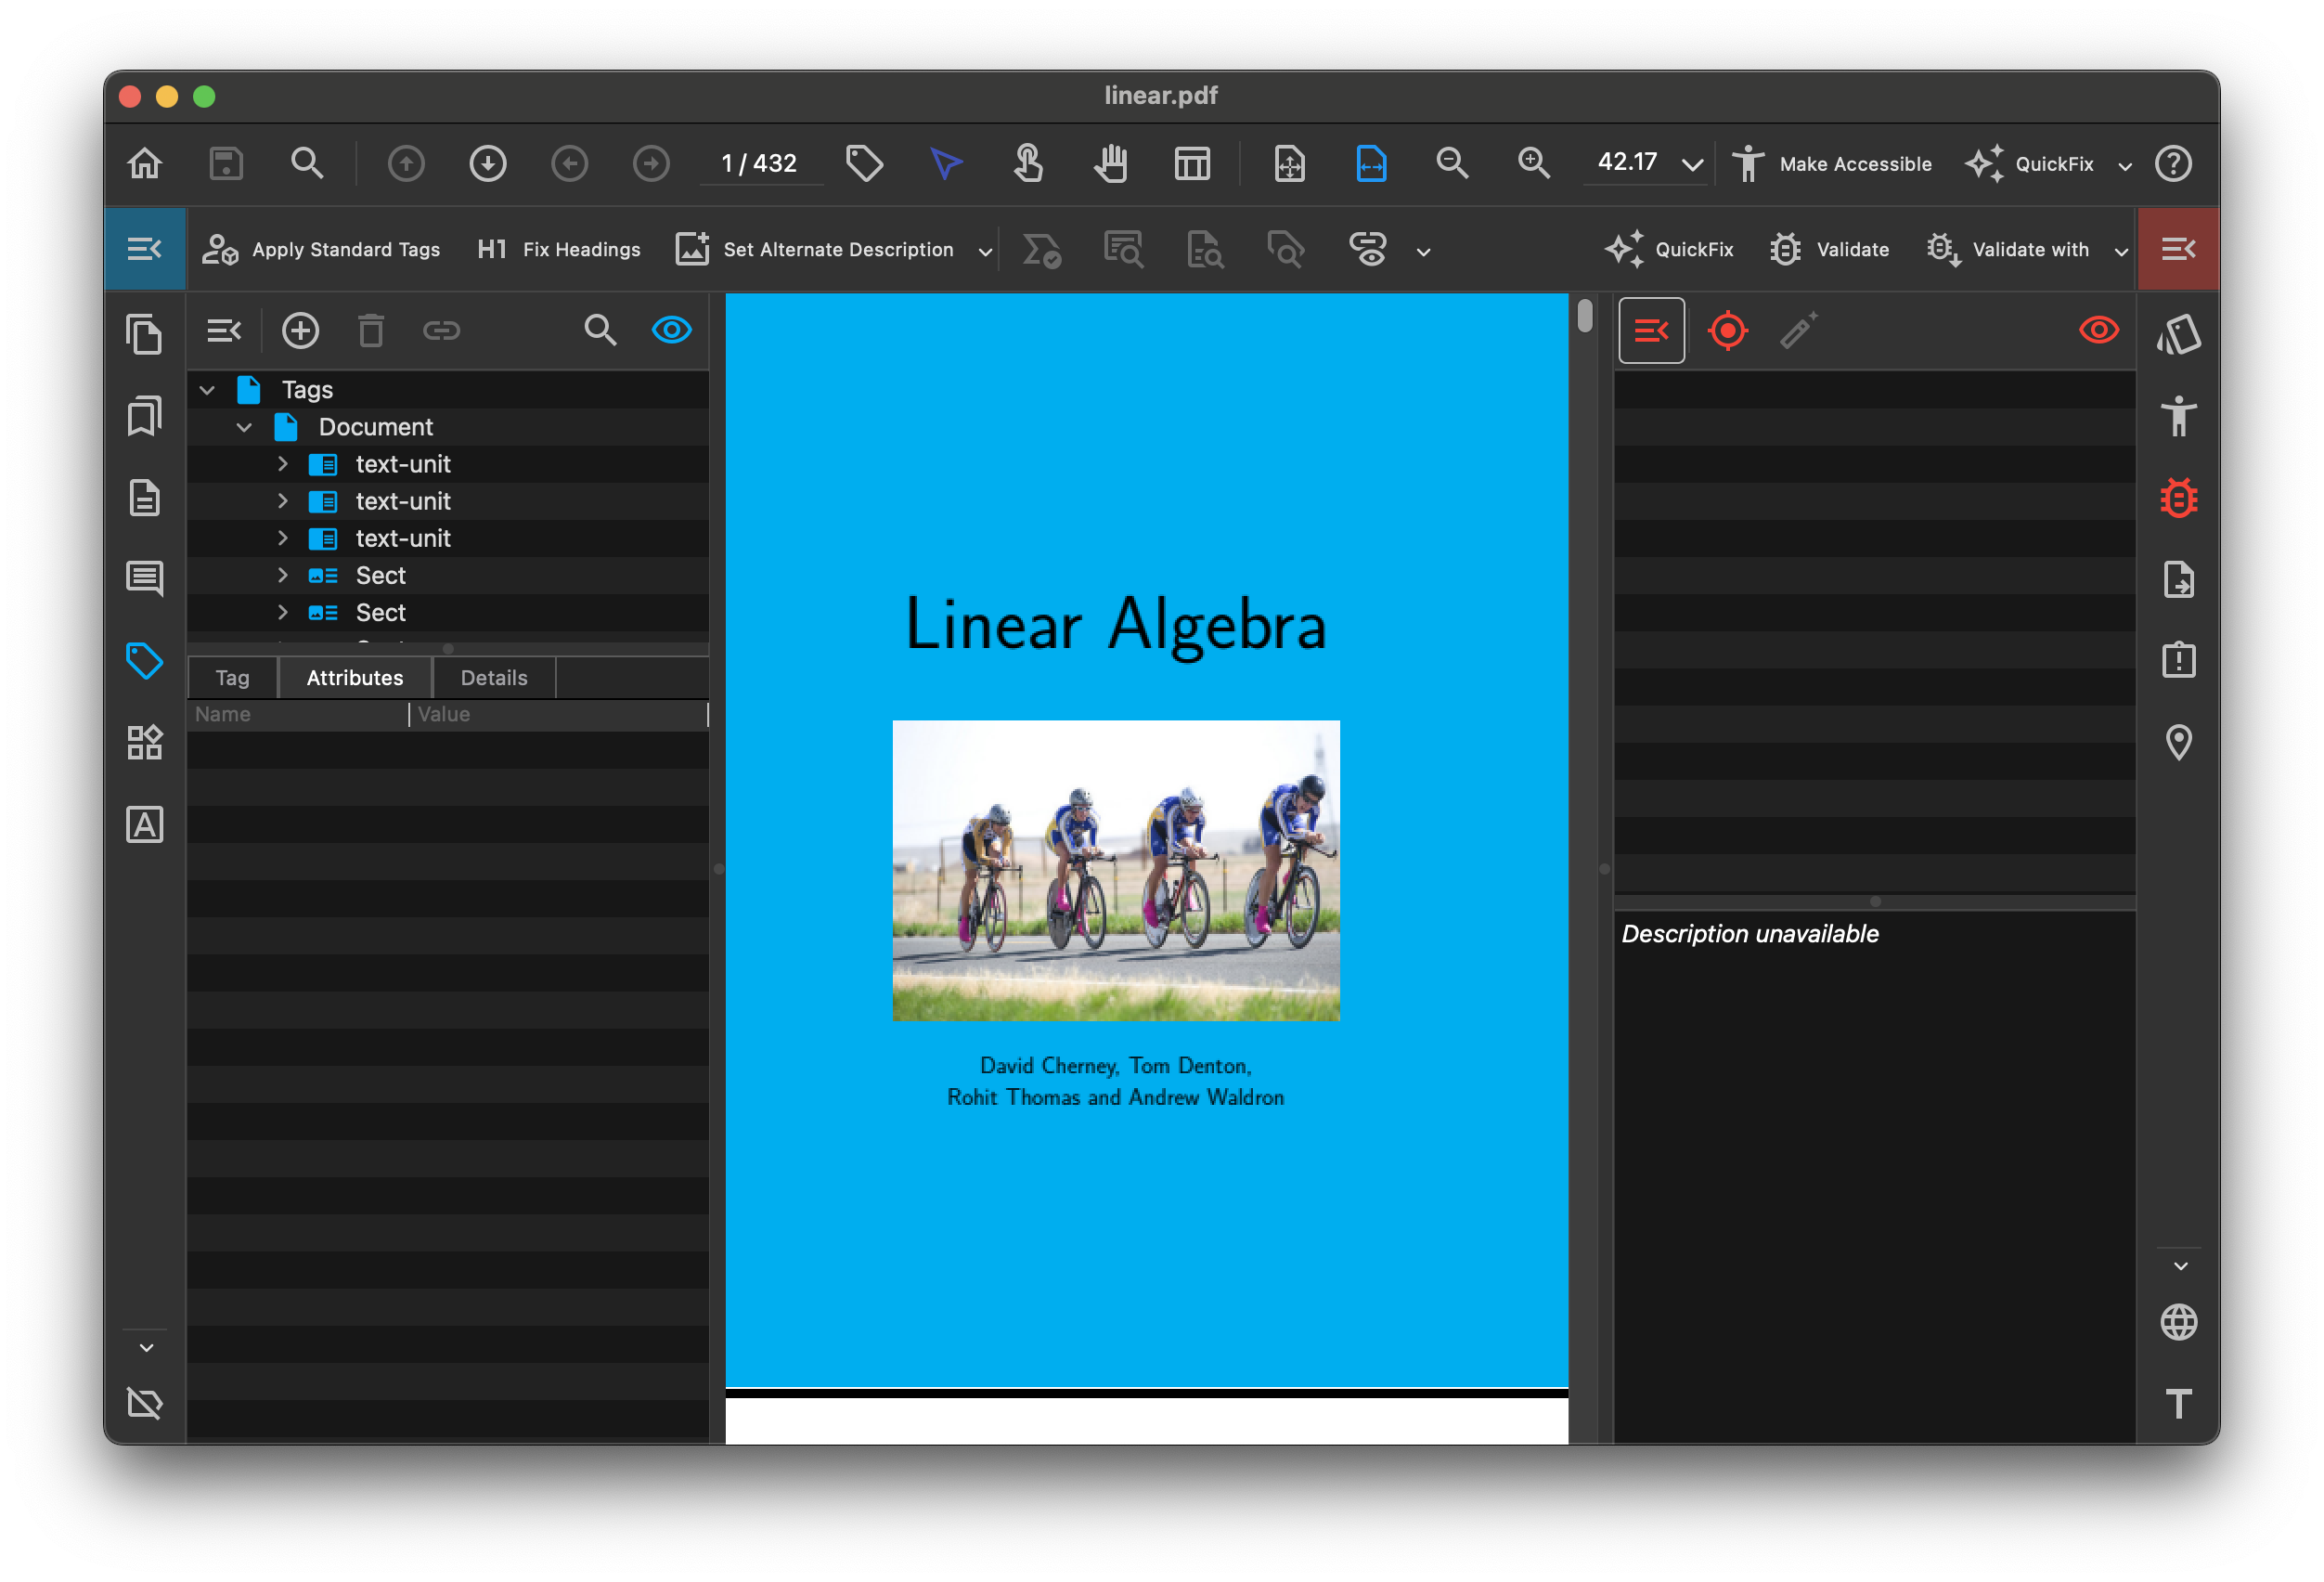
\includegraphics[alt={Screenshot of PDFix},height=\textheight]{pdfixScreenshot}
\end{frame}

\begin{frame}
\frametitle{PDFix --- same example error}
%\centering
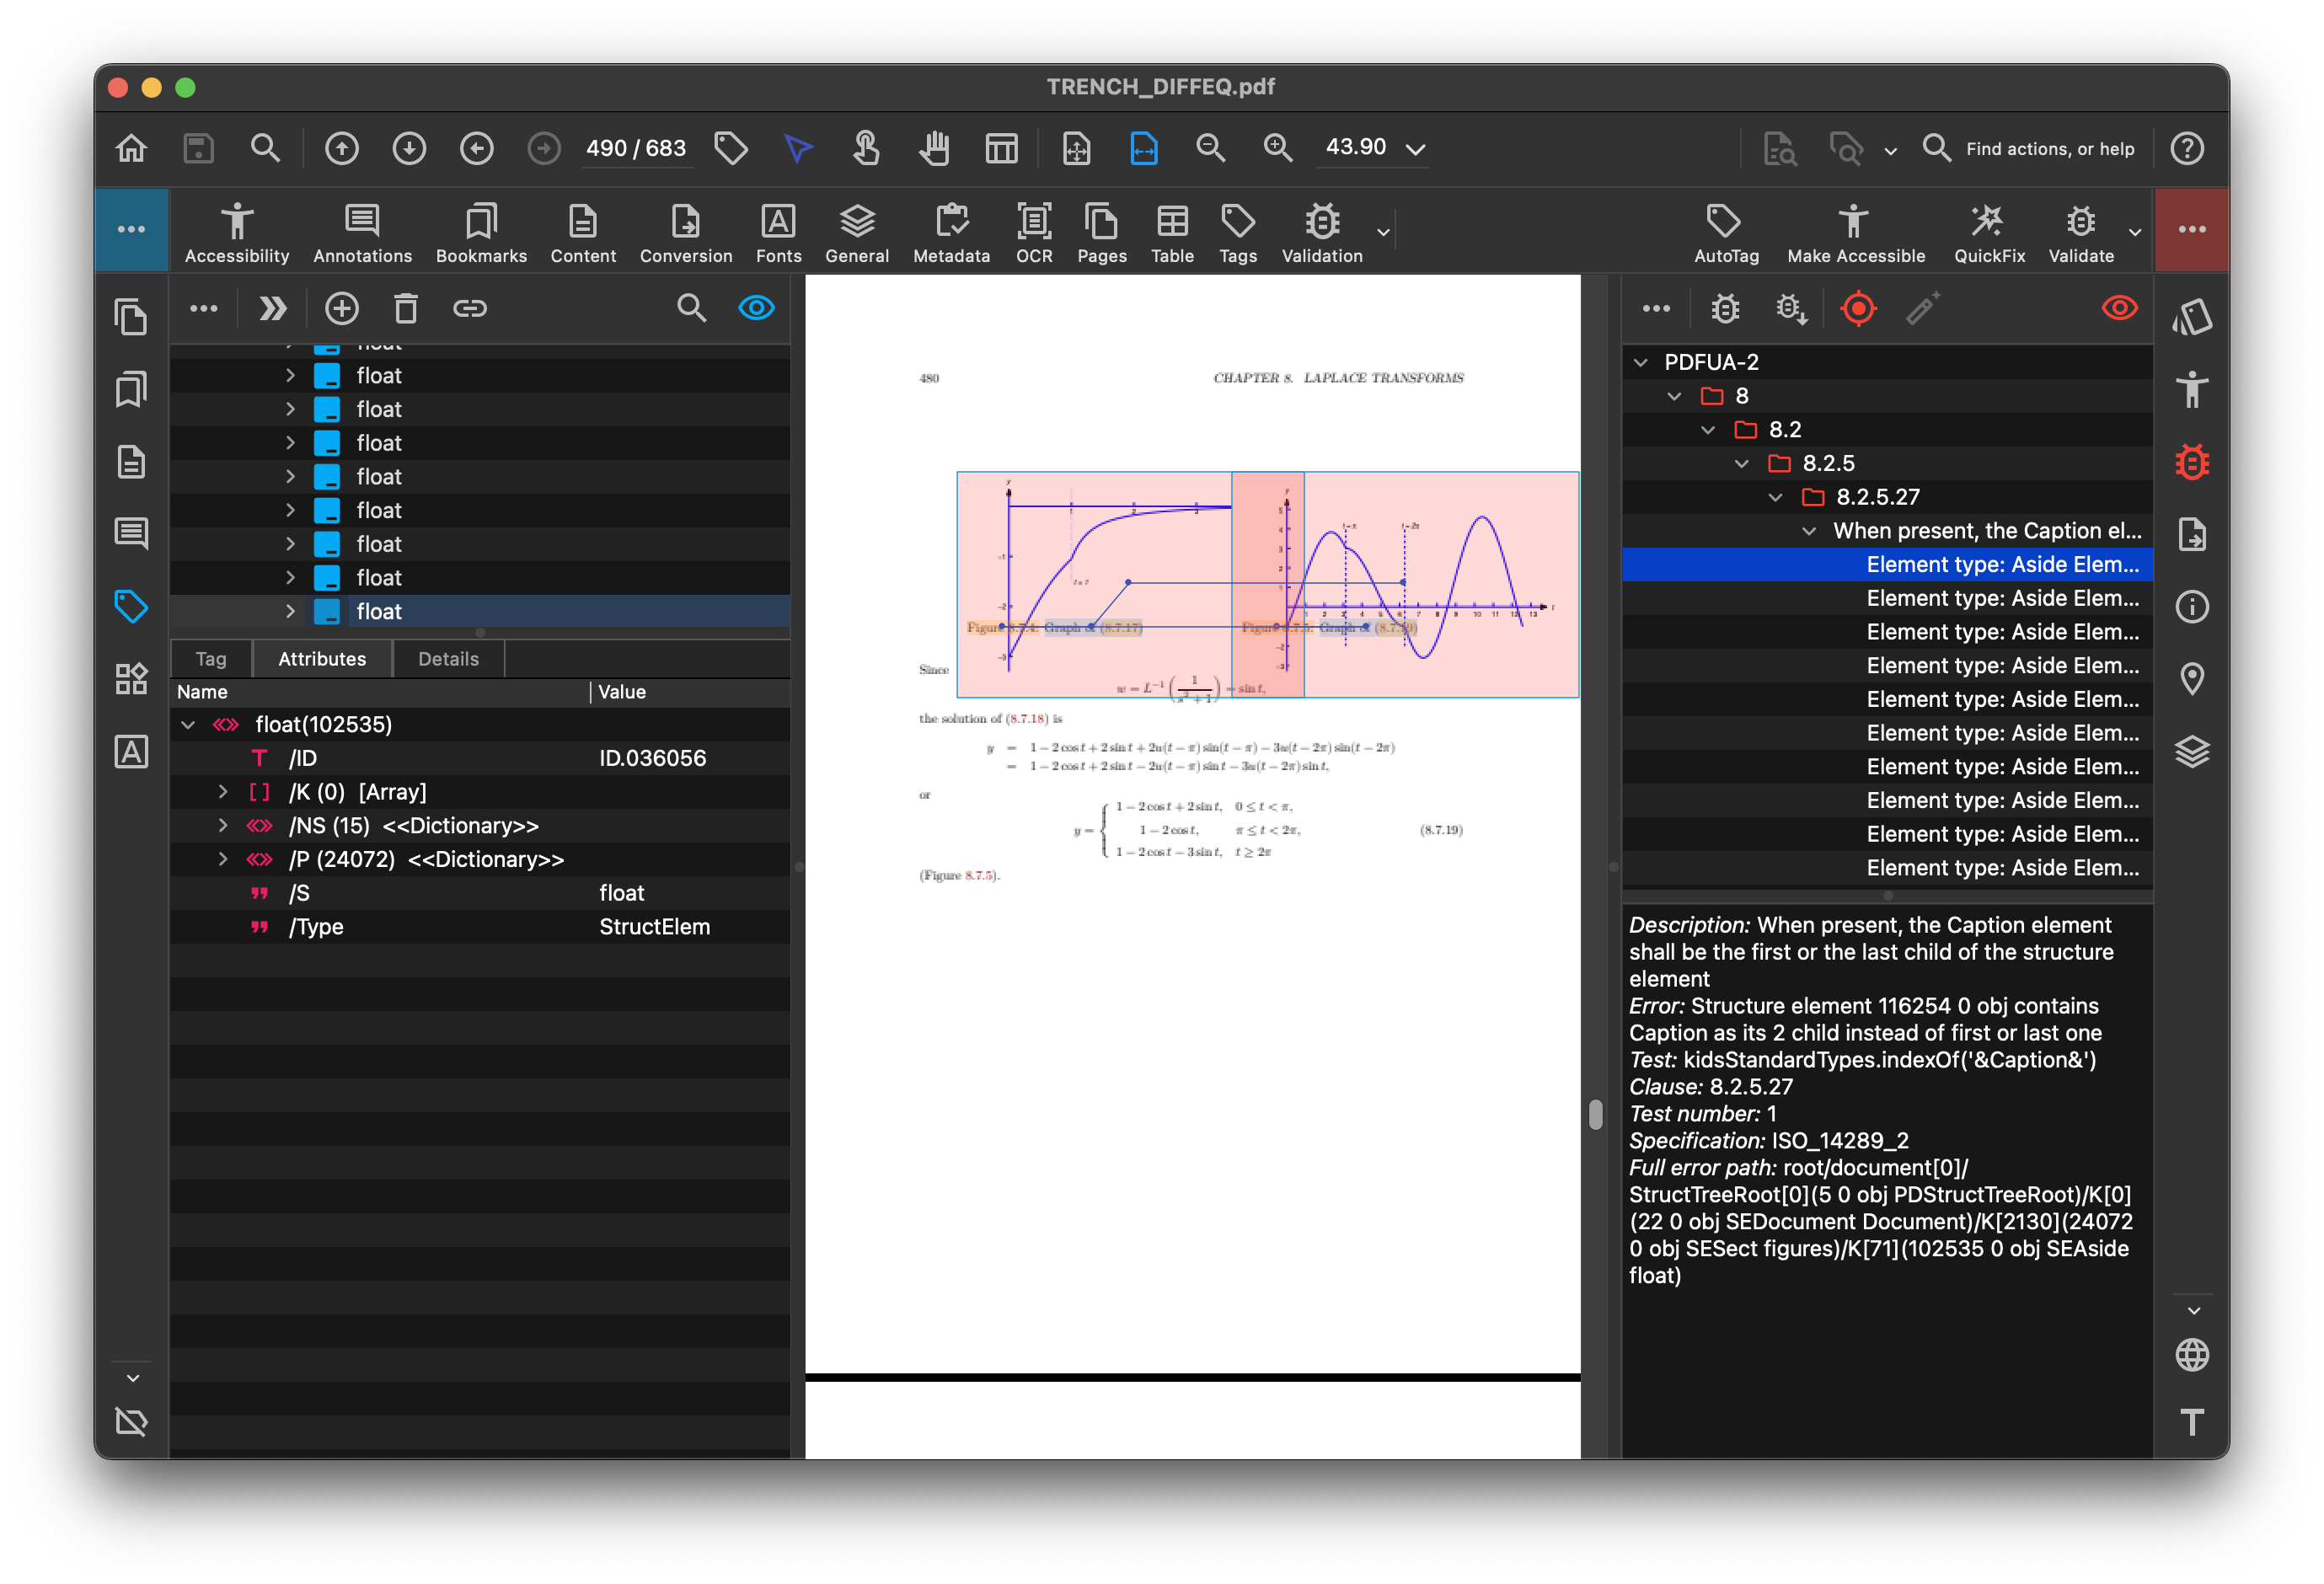
\includegraphics[alt={Screenshot of PDFix error},height=\textheight]{pdfixValError}
\end{frame}

%\begin{frame}
%\frametitle{PAC --- \url{https://pac.pdf-accessibility.org/en}}
%\centering
%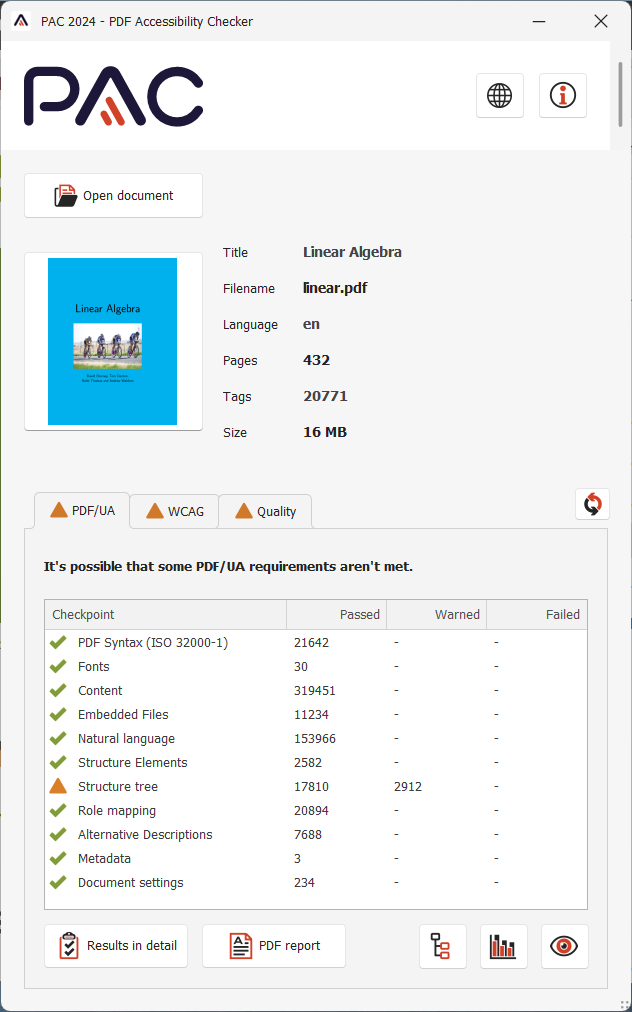
\includegraphics[alt={Screenshot of PAC},height=\textheight]{PacScreenshot}
%\qquad
%\raisebox{.5\textheight}{\parbox{.5\linewidth}{A bit more streamlined, but:
%\begin{itemize}
%\item Windows only
%\item maxes out at UA-1/1.7
%\item objects to bug in pgfplots
%\item has a bug with tables
%\item doesn't like multi(row/column)
%\end{itemize}
%\end{frame}

%\begin{frame*}
%\frametitle{ltx-talk}\pause
%\begin{itemize}[<+->]
%\item Same \verb|\pause|/overlay specification idea (eg, \verb|\begin{itemize}[<+->]|)
%\item ``\emph{highly} experimental'' --- must use \texttt{lualatex-dev} (for another month?)
%\item Ally $\Rightarrow$ \verb|\AtBeginDocument{\tagpdfsetup{role/new-tag=frametitle/H1}}|
%\item Can ``easily'' specify header and footer information\\\bigskip
%\hfill%
%\alt<+->{%
% 
\includegraphics[height=.4\textheight,alt={MALL presentation with logo in corner}]{Blackboard-PPT-Tues.pdf}%
%}{%
% \parbox[c][.4\textheight]{1em}{}%
%}%
%\hfill\null
%\end{itemize}
%\end{frame*}

%\section{For more information}

\begin{frame}
\renewcommand{\ULthickness}{2pt}
\frametitle{Misconceptions}
Email from IT:
\begin{quote}
%\!\!``
\makebox[0pt][r]{``}%
% [PDF] == the format that it is in now
To keep it in [PDF] would result in major \alert<2>{clean-up} to the tagging structure (\alert<2>{in Adobe} particularly). You could do it, but 1000 pages \alert<2>{in Adobe} is a lot \alert<2>{to remediate}. Additionally, the code in the content tab of Adobe has a lot of \alert<3>{rogue elements} that came over. There are \alert<3>{containers in there that don't even correspond to textual or visual elements on the page}, so I don't know where those came from; they must have resulted from something in the conversion process from LaTex to PDF.''
\end{quote}\bigskip
\begin{itemize}
\item \alert<2>{\texttt{.tex} $\overset{\texttt{lualatex}}{\to}$}
\alt<2>{%
 {\alert{%
  \sout{\color{black}%
  \texttt{.pdf}
  \color{black}%
  $\overset{\text{Adobe}}{\to}$}%
 }}%
}{%
  \texttt{.pdf}
  $\overset{\text{Adobe}}{\to}$%
}
\alert<2>{\texttt{.pdf\,2.0}}
is \alt<2>{\alert{\sout{\color{black}not}}}{not} a viable process
\item<1-|alert@2> Remediation can be done at creation by \LaTeX, not after in Adobe
\item<1-|alert@3> Adobe checks \texttt{PDF\,1.7}, not \texttt{PDF\,2.0}
\end{itemize}
\end{frame}

\begin{frame*}
\frametitle{Last bits}
\begin{itemize}
\item \url{https://latex3.github.io/tagging-project}
\item \url{https://github.com/teepeemm/accessibility}
\item Compiling needs more:\medskip\\
\quad
\begin{tabular}{l @{\qquad} S[table-format=2(1),uncertainty-mode=separate]}\toprule
Statistic & Factor \\\midrule
Time & 10(3) \\
RAM & 6(2) \\
Output size & 2(1) \\
strings & 11(4)\\
hash & 10(4)\\\bottomrule
\end{tabular}
\medskip\\
Use \verb|\DocumentMetadata{tagging=off}| for draft runs
%\item \url{https://www.youtube.com/watch?v=Eu_qM53tInw&t=5900s}\\
%\qquad A before and after example using Foxit, NVDA, and MathCAT
\item Don't be afraid to edit beyond the preamble
\end{itemize}
\end{frame*}

%\end{document}
%
%\begin{frame}
%\frametitle{Examples}\tagpdfsetup{table/header-rows={1}}
%\begin{tabular}{l p{.2\textwidth} p{.5\textwidth}}
%Math & before & after \\\midrule
%$a^2+b^2=c^2$ & ay two plus bee two equals cee two & ay squared plus bee squared is equal to cee squared\\\addlinespace[4ex]
%{$\begin{pmatrix}a&b\\c&d\end{pmatrix}^{-1}$} & minus one list with one item ay bee cee dee & two lines line one ay bee line two cee dee to the negative one power \\\addlinespace[4ex]
%{$\begin{pmatrix}1&2\\3&4\end{pmatrix}\begin{pmatrix}1&1\\0&1\end{pmatrix}$} & three four one two zero one one one & the two by two matrix row one one two row two three four times the two by two matrix row one one one row two zero one
%\end{tabular}
%\end{frame}

% cut for MAA
%\begin{frame}
%\frametitle{Colors}
%\begin{itemize}
%\item UND green is $\operatorname{RGB}(0,158,68)=\operatorname{Hsb}(146,1,0.62)$
%\item UND orange is $\operatorname{RGB}(255,103,31)=\operatorname{Hsb}(19,0.88,1)$
%\item Insufficient contrast with white?
%\item Add 13\% and 22\% black.
%\item Also red with white (hyperref)
%\end{itemize}
%\end{frame}

\title{Convert\makebox[0pt][l]{\raisebox{.6\baselineskip}{\color{alert}ed}}{\color{alert}\sout{\color{structure}ing}} a PDF Textbook to be Accessible}

\reuseframe{titleslide}

\begin{frame}\thispagestyle{empty}
\end{frame}

%%%%%%%%%%%%%%%%%%%%%%%%%%%%%%%%%%%%%%%%%%%%%%%%%%

\title[Accessible Presentations]
 {Creating Accessible Presentations With \texttt{ltx-talk}}
\subtitle{beamer+tagging}

\reuseframe{titleslide}

\reuseframe<2>{stycls}

\begin{frame*}
\frametitle{The basics}
\begin{itemize}
\item
\begin{lstlisting}
\DocumentMetadata{
  lang=en,
  tagging=on,
  pdfstandard=ua-2,
%  check-tagging-status,
  tagging-setup={
%    math/alt/use,               % <=> Formulas must have description/alt text
%    role/new-tag=frametitle/H1, % <=> headings must begin at level 1
    math/setup=mathml-SE
  }
}
\documentclass{ltx-talk}
\end{lstlisting}
\item Lua\LaTeX
\item defined colors: \textcolor{alert}{alert}, \textcolor{example}{example}, \textcolor{structure}{structure}
\item \tubbraced{frame*} $\Leftrightarrow$ \verb@\verb|...|@,
\tubbraced{verbatim}, \tubbraced{lstlisting}, etc. (like Beamer's \texttt{fragile})
\item tagged PDF + overlays: \verb|\command<xyz>| \textrightarrow\ \cs{command} only on slides \verb|xyz|
\end{itemize}
\end{frame*}

% maybe cut this
\begin{frame*}<-5>
\frametitle{More basics --- overlays (slide \arabic{slide})}
Overlays: \verb|\command<xyz>| \textrightarrow\ \cs{command}
only on slides \verb|xyz|%\bigskip
\begin{itemize}
\item Color commands with overlays: \cs{color}, \cs{mathcolor}, \cs{textcolor},
\textcolor{structure}{\Large\star} \alert{\cs{alert}}
\item Text commands with overlays: \cs{textbf}, \cs{textit},
\cs{textmd}, \cs{textnormal}, \cs{textrm}, \cs{textsc}, \cs{textsf}, \cs{textsl}, \cs{texttt}, \cs{textup},
\cs{emph}
\item Also: \cs{includegraphics}; \cs{label}
\item \verb|\alt<2>{
\includegraphics{alt}}|\hphantom{\ttfamily East VillageXX}
\alt<2>
 {\raisebox{-\baselineskip}[0pt][0pt]{%
   
\includegraphics[alt={Alt Hotel Logo},height=2\baselineskip]{alt}}}
 {\raisebox{-.5\baselineskip}[0pt][0pt]{Alt Hotel, Calgary East Village}}%
\\
 \hphantom{\ttfamily XaltX2X}\verb|{Alt Hotel, Calgary East Village}|
\item
\setkeys{Gin}{height=6\baselineskip}
\verb|\temporal<4>{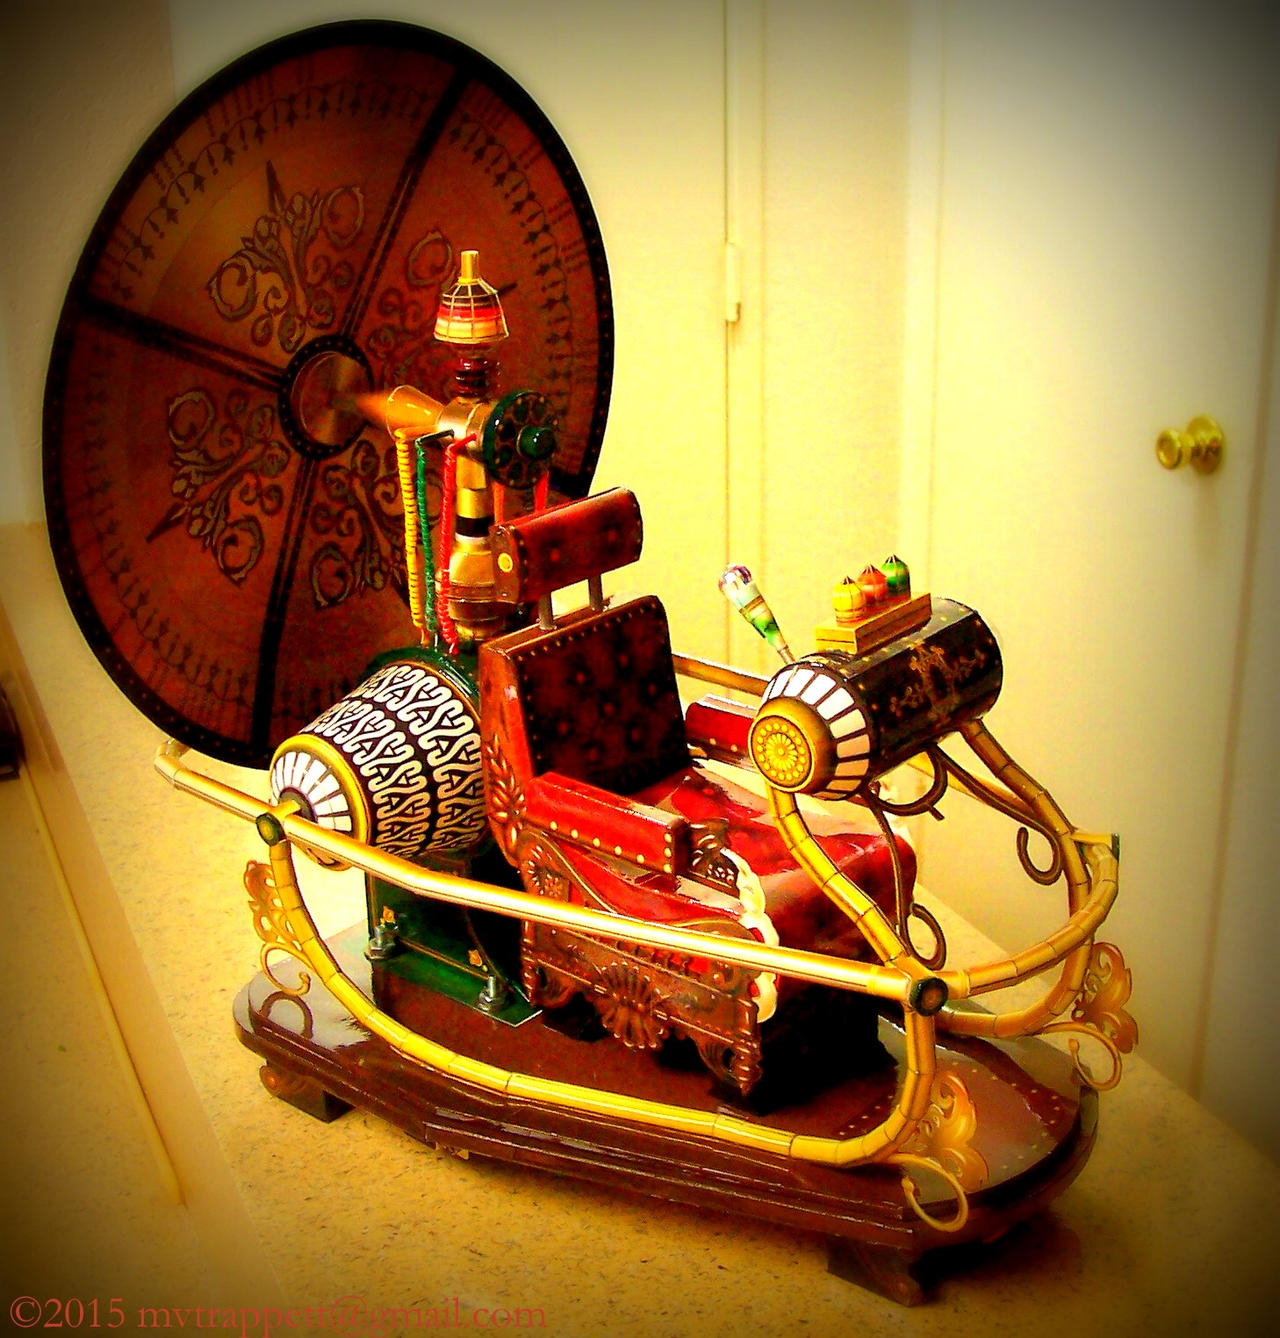
\includegraphics{before}}|\hspace{3cm}
\raisebox{-5\baselineskip}[0pt][0pt]{%
\temporal<4>
 {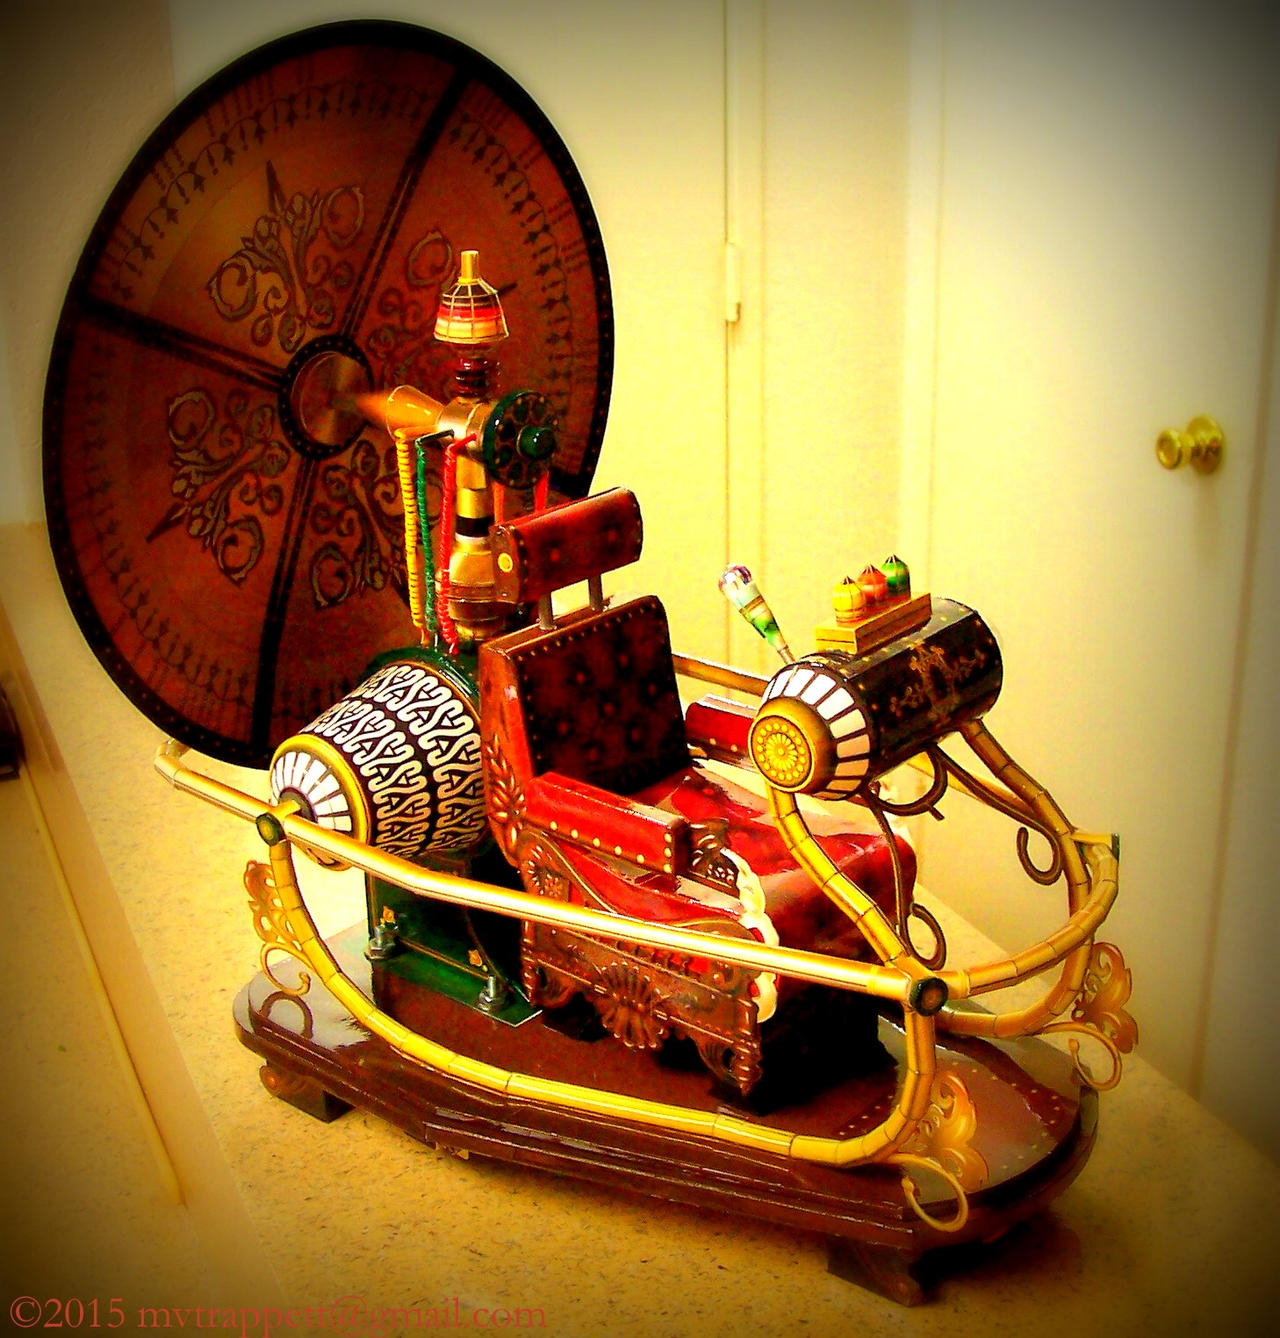
\includegraphics[alt={early time travel}]{before}}
 {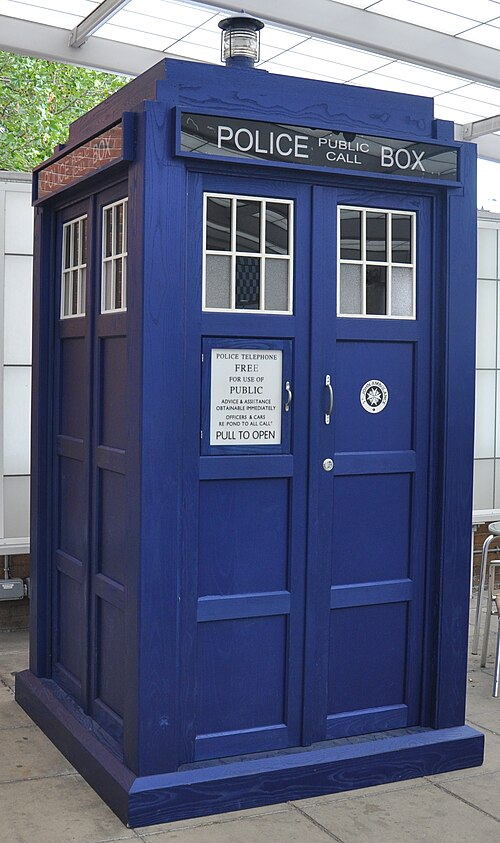
\includegraphics[alt={contemporary time travel}]{current}}
 {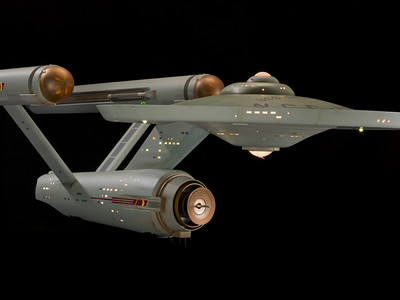
\includegraphics[alt={futuristic time travel}]{after}}%
}
 \\
\hphantom{\ttfamily XtemporalX2X}\verb|{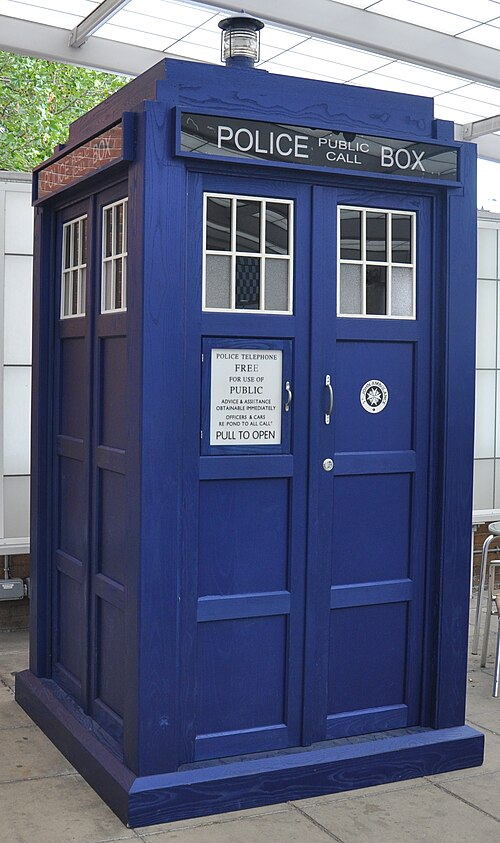
\includegraphics{current}}|\\
\hphantom{\ttfamily XtemporalX2X}\verb|{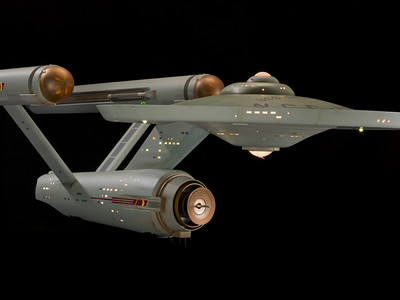
\includegraphics{after}}|
\item[\Large\star] \cs{only}, \cs{uncover}, \cs{visible}, \cs{invisible}
%, \cs{alert}
%\item \verb|\onslide<2>{
\includegraphics{onslide}}|: \onslide<2>{
\includegraphics{onslide}}
\item \cs{item}, \cs{action}, \tubbraced{actionenv} can take an
\emph{action specification}\\
(combine several \textcolor{structure}{\Large\star} actions
into one \verb|<...>|)
\item Environments \tubbraced{onlyenv}, \tubbraced{invisibleenv},
\tubbraced{uncoverenv}, \tubbraced{visibleenv}, \tubbraced{alertenv}
%\item Also: \cs{item} (and can take an \emph{action spec})
%\item Main overlay commands: \cs{onslide}, \cs{only}, \cs{uncover}, \cs{visible}, \cs{invisible}, \cs{alt}, \cs{temporal}
%\item Overlay environments: \tubbraced{onlyenv}, \tubbraced{invisibleenv}, \tubbraced{uncoverenv}, \tubbraced{visibleenv}
\end{itemize}
\end{frame*}

% maybe cut this
\begin{frame*}
\frametitle{Overlays}
To define an overlay command:
\begin{lstlisting}
\NewDocumentCommand{\mycommand}{ s D<>{1-} ... }{ ...}

% or

\NewDocumentCommand{\mycommand}{ s d<> ... }{ ...}
\end{lstlisting}
%For example
%\begin{lstlisting}
%\NewDocumentCommand{\visablealert}{ d<> m }{%
% \visible<#1->{\alert<#1>{#2}}}
%\end{lstlisting}
\end{frame*}

\begin{frame}
\frametitle{Sectioning}
\begin{itemize}
\item \sout{\cs{part}}, \sout{\cs{chapter}},\\
\cs{section}, \cs{subsection}, \cs{subsubsection},\\
\sout{\cs{paragraph}}, \sout{\cs{subparagraph}}
\item (currently?) no visible output\\
\qquad only affects the \cs{tableofcontents} (and bookmarks and tagging)\\
\qquad when used outside of frames
\end{itemize}
\end{frame}

\begin{frame}<1>[name=TOCslide,tag-slides=1-2]
\frametitle{A \cs{tableofcontents}\only<2>{ in a \cs{((sub)sub)section}}}
\begin{multicols}{2}
\setcounter{tocdepth}{3}
\tableofcontents
\end{multicols}
\hrule\bigskip
Default \texttt{tocdepth} is 2 (\cs{subsection}).
\end{frame}

\section{Accessible Textbook}
\subsection{Preamble}
\subsection{Images}
\subsection{Tables}
\subsection{All else}
\subsection{Tools}
\addtocontents{toc}{\protect\columnbreak}
\section{Accessible Presentations}
\subsection{The basics}
\subsection{Sectioning}

\reuseframe<2>{TOCslide}

\subsection{Examples}

\subsubsection{List environments}

\begin{frame*}
\frametitle{List environments}
\begin{itemize}
\item \tubbraced{itemize}, \tubbraced{enumerate}, \tubbraced{description}
as in \LaTeX
\item templates mean we can pass options to the environments,\\
see \texttt{texdoc blocks-doc}
\item extra (default) key \texttt{action-spec}
\item \verb!action-spec=<+->! \qquad uncover one item at a time % hspace
\item \verb!action-spec=<+-|alert@+>!
\qquad and \alert{\cs{alert}} the new item
\end{itemize}
\end{frame*}

\newlength\mylabelwidth
\setlength\mylabelwidth{\widthof{tagged PDFs}}
\begin{frame*}
  \frametitle{A strangely sporadic glossary}
 \begin{minipage}{.54\textwidth}
 \lstset{aboveskip=0pt,belowskip=0pt}
 \begin{lstlisting}
\newlength\mylabelwidth
\setlength\mylabelwidth{\widthof{tagged PDFs}}
\begin{frame}
 \frametitle{A strangely sporadic glossary}
\end{lstlisting}
\lstinputlisting{exampleDesc}%
\begin{lstlisting}
\end{frame}
\end{lstlisting}
 \end{minipage}%
 \begin{minipage}{.46\textwidth}
 \begin{description}[
  label-align=left,
  label-width=\mylabelwidth+0.5em,
  left-margin=\mylabelwidth+1em,
  action-spec=<+->, ]
  \item[\LaTeX] \TeX\ and one or two
   additional macros
  \item[\texttt{beamer}] presentation
   class for \LaTeX
  \item[tagged PDFs] Computers can read PDFs
  \item[\texttt{ltx-talk}] tagged
   \texttt{beamer} PDF
 \end{description}

\end{minipage}
\end{frame*}

\begin{frame*}<1>[name=usewhich,tag-slides={1-2}]
\frametitle{Which slides to use?}
\begin{itemize}
\item Which slides should a screen reader use?
\item Default is the last slide: \texttt{tag-slides=n}
\item<2> Previous example: \texttt{tag-slides=\{1-\}}\bigskip
\item Which slides should\\
\verb|\documentclass[mode=handout]{ltx-talk}| use?
\item Default is to ignore all overlays and just use slide \texttt{n}
\item<2> Fails in previous example: everything alerted\\
\verb#<projector:(spec)|handout:(spec)># for the handout to have everything\\
\verb#<projector:(spec)|article># for the handout to have last slide only
%\newcommand{\colvect}[1]{%
% \begin{pmatrix}#1\end{pmatrix}}
%\[\alert{
%  \colvect{1\\2}
%  \colvect{4\\5}
%  \bullet
%  \colvect{-2\\2}
%  \colvect{4\\-5}
%  =
%  2-62-9
%}\]
\end{itemize}
\end{frame*}

\subsubsection{Interesting use of overlays}

\begin{frame*}[tag-slides={1-}]
\lstset{aboveskip=0pt,belowskip=0pt}
\frametitle{Matrix multiplication example,
 step \arabic{slide}}
 \begin{minipage}{.57\textwidth}
 %
 \begin{onlyenv}<1>
\begin{lstlisting}
\begin{frame}[tag-slides={1-}]
 \frametitle{Matrix multiplication example,
  step \arabic{slide}}
\end{lstlisting}
 \end{onlyenv}
 %
 % exampleMatrix.tex has 29 lines of content
 \only<1>{\lstinputlisting[lastline=16]{exampleMatrix}}\par
 \only<2>{\lstinputlisting[lastline=19]{exampleMatrix}}\par
 \only<3>{\lstinputlisting[firstline=4,lastline=22]{exampleMatrix}}\par
 \only<4>{\lstinputlisting[firstline=7,lastline=25]{exampleMatrix}}\par
 \only<5>{\lstinputlisting[firstline=10,lastline=28]{exampleMatrix}}\par
 \only<6>{\lstinputlisting[firstline=12]{exampleMatrix}}
 %
 \begin{onlyenv}<6>
 \begin{lstlisting}
\end{frame}
\end{lstlisting}
\end{onlyenv}
%
\end{minipage}%
\begin{minipage}{.43\textwidth}
\begin{gather*}
\begin{pmatrix}
\alert<2,3>{1}&\alert<2,3>{2}\\
\alert<4,5>{4}&\alert<4,5>{5}
\end{pmatrix}
\begin{pmatrix}
 \alert<2,4>{-2}&\alert<3,5>{ 4}\\
 \alert<2,4>{ 2}&\alert<3,5>{-5}
\end{pmatrix}
\visible<2-6>{
 {}=\begin{pmatrix}
  \uncover<2->{\alert<2>{ 2}}&
  \uncover<3->{\alert<3>{-6}}\\
  \uncover<4->{\alert<4>{ 2}}&
  \uncover<5->{\alert<5>{-9}}
 \end{pmatrix}}
\\[\bigskipamount]
\vphantom{\begin{pmatrix}1\\2\end{pmatrix}}%
\invisible<1,6>{
 \alert{
  \only<2,3>{\begin{pmatrix}1\\2\end{pmatrix}}
  \only<4,5>{\begin{pmatrix}4\\5\end{pmatrix}}
  \bullet
  \only<2,4>{\begin{pmatrix}-2\\ 2\end{pmatrix}}
  \only<3,5>{\begin{pmatrix} 4\\-5\end{pmatrix}}
  =
  \only<2>{\phantom-2}\only<3>{-6}
  \only<4>{\phantom-2}\only<5>{-9}}}
\end{gather*}

\end{minipage}
\end{frame*}
% see https://github.com/josephwright/ltx-talk/issues/234

\reuseframe<2>{usewhich}

\subsection{Customizations}

\subsubsection{Adjusting the header}

\begin{frame*}
\frametitle{Adjusting the header}
\begin{columns}[vertical-alignment=top]%
\begin{column}{.45\textwidth}%
\verb|\EditInstance{header}{std}|\\
\hphantom{\ttfamily XEditInstance}\verb|{<key=value>}|
%or
\\
\medskip
\begin{tabular}{ ll }\toprule
Key & Default Value\\\midrule
background-color & (none)\\
color & \color{structure}structure \\
font & \cs{normalfont}\\
height & topmargin (\qty{10}{mm})\\
 & \quad+ headsep (\qty2{mm})\\
left-hspace & leftmargin (\qty{10}{mm})\\
right-hspace & rightmargin (\qty{10}{mm})\\
print-frame-title & true\\\bottomrule
\end{tabular}
\end{column}%
\begin{column}{.1\textwidth}\makebox[\linewidth][c]{or}\end{column}%
\begin{column}{.45\textwidth}%
\verb|\EditInstance{frametitle}{header}|\\
\hphantom{\ttfamily XEditInstance}\verb|{<font=value>}|
\\\medskip
\begin{tabular}{ ll }\toprule
Key & Default Value\\\midrule
before-vspace & 0em \\
after-vspace & bigskip (12pt±4pt)\\
color & (none) \\
font & \cs{Large}\cs{bfseries}\\\bottomrule
\end{tabular}
\end{column}
\end{columns}
\end{frame*}

%\showthe\bigskipamount -> 12pt + 4pt - 4pt

%>  after-vspace  =>  \bigskipamount 
%>  before-vspace  =>  0em
%>  color  =>  
%>  font  =>  \Large \bfseries 

\begin{frame*}
\frametitle{A logo in the header
$\qquad\longrightarrow\qquad\longrightarrow$}
\begin{lstlisting}
\newsavebox\logobox
\savebox\logobox{%
  \includegraphics[artifact, height=\baselineskip]{logo-file}%
}

% after \maketitle frame
\AddToHook{shipout/foreground}{%
  \put(\paperwidth - \wd\logobox - 10mm,
       -8.5mm){\usebox\logobox}% -\ht\logobox
}
\end{lstlisting}
\end{frame*}
%\NewCommandCopy\oldframetitle\frametitle
%\RenewDocumentCommand{\frametitle}{m}{%
%  \oldframetitle{#1\hfill
%    \includegraphics[height=2ex,artifact]{logo-file}%
%  }%
%}

\subsubsection{Adjusting the footer}

\begin{frame*}
\frametitle{Adjusting the footer}
\verb|\EditInstance{footer}{std}{<key=value>}|\\\medskip
\begin{tabular}{ll}\toprule
Key & Default Value\\\midrule
background-color & (none)\\
color & black \\
element-order & (empty)\\
font & \cs{tiny}\\
left-hspace & leftmargin (\qty{10}{mm}) \\
right-hspace & rightmargin (\qty{10}{mm}) \\
separator & \cs{hfil}\\\bottomrule
\end{tabular}\\\medskip
Available footer elements:\\
author, date, institute, title, subtitle, framenumber,
totalframes (=\cs{RefProperty}\tubbraced{lastpage}\tubbraced{totalframes})\\
For example:
\verb|\EditInstance{footer}{std}{element-order={date,author,title,framenumber}}|
\end{frame*}

\begin{frame*}
\frametitle{Creating a custom footer element}
\lstset{aboveskip=0pt,belowskip=0pt}
\begin{lstlisting}
\DeclareInstance{footer-element}{myelement}{talk}{...}
% and then
\makeatletter
\newcommand\@myelement{...}
% or
\newcommand\@shortmyelement{...}                 % used if both available
\makeatother
% or
\ExpandArgs{c}\newcommand{@myelement}{...}
% or
\ExpandArgs{c}\newcommand{@shortmyelement}{...}  % used if both available
\end{lstlisting}
and then pass \texttt{myelement} to \texttt{element-order}\\
For example:
\begin{lstlisting}
\ExpandArgs{c}\newcommand{@framesoftotal}{%
 \arabic{frame}/\RefProperty{lastpage}{totalframes}%
}
\end{lstlisting}
\end{frame*}

\subsubsection{Adjusting the title page}

\begin{frame*}
\frametitle{Default title page}
\begin{columns}
\begin{column}{.5\textwidth}
\begin{lstlisting}
\maketitle

% same as

\maketitle[
  element-order        = {
    title, subtitle, author,
    institute, date
  },
  framestyle           = talk,
  horizontal-alignment = center,
  vertical-alignment   = center
]
\end{lstlisting}
\end{column}
\begin{column}{.5\textwidth}
\maketitle
\end{column}
\end{columns}
\end{frame*}

\begin{frame*}
\frametitle{Adjusting the title page}
\begin{columns}
\begin{column}{.5\textwidth}
Adjusted title page:
\begin{lstlisting}
\maketitle[
  element-order = {
    title, author,
    titlegraphic, date
  },
  framestyle    = plain,
]
\end{lstlisting}
\cs{thispagestyle}\tubbraced{framestyle}
options:% \texttt{talk}, \texttt{plain} \& \texttt{wallpaper}
\begin{description}
\item[talk] default header and footer
\item[plain/empty] no header and footer
\item[wallpaper] header and footer have\\
 background color but no text
\end{description}
\end{column}
\begin{column}{.5\textwidth}
\maketitle[
  element-order = {title, author, titlegraphic, date},
  framestyle = plain,
]
\end{column}
\end{columns}
\end{frame*}

\begin{frame*}
\frametitle{Creating a custom title element}
\lstset{aboveskip=0pt,belowskip=0pt}
\begin{lstlisting}
\DeclareInstance{titlepage-element}{myelement}{talk}{<key=value>}
% and then
\makeatletter
\newcommand\@myelement{...}
\makeatother
% or
\ExpandArgs{c}\newcommand{@myelement}{...}
\end{lstlisting}
and then pass \texttt{myelement} to \cs{maketitle}'s \texttt{element-order}\\
For example:
\begin{lstlisting}
\ExpandArgs{c}\newcommand{@titlegraphic}{%
  \includegraphics[
    actualtext={University of North Dakota, Mathematics \& Statistics},
    width=5cm
  ]{graphic-file}%
}
\end{lstlisting}
\end{frame*}

\subsubsection{More customizations}

\begin{frame*}
\frametitle{More customizations}
\begin{lstlisting}
\EditInstance{floatenv}{std}{horizontal-alignment = <alignment>}
% left (default), center, or right

\EditInstance{hidden}{std}{opacity = <value>}
% 0 <= value <= 1 for how opaque hidden things should be
% default is 0
\end{lstlisting}
\end{frame*}

\subsection{Future work}

\begin{frame}
\frametitle{Future work}
\begin{itemize}
\item tagging
\begin{itemize}
\item blocks
\item heading structure
\item sectioning
\end{itemize}
\item frame layout
\begin{itemize}
\item header / footer templates
\item frame title
\end{itemize}
\end{itemize}
\end{frame}

\title{Creat\makebox[0pt][l]{\raisebox{.6\baselineskip}{\color{alert}ed}}{\color{alert}\sout{\color{structure}ing}} Accessible Presentations With \texttt{ltx-talk}}

\reuseframe{titleslide}

\end{document}
